  \let\negmedspace\undefined
\let\negthickspace\undefined
\documentclass[journal]{IEEEtran}
\usepackage[a5paper, margin=10mm, onecolumn]{geometry}
\usepackage{lmodern} % Ensure lmodern is loaded for pdflatex
\usepackage{tfrupee} % Include tfrupee package

\setlength{\headheight}{1cm} % Set the height of the header box
\setlength{\headsep}{0mm}     % Set the distance between the header box and the top of the text

\usepackage{gvv-book}
\usepackage{gvv}
\usepackage{cite}
\usepackage{amsmath,amssymb,amsfonts,amsthm}
\usepackage{algorithmic}
\usepackage{graphicx}
\usepackage{textcomp}
\usepackage{xcolor}
\usepackage{txfonts}
\usepackage{listings}
\usepackage{enumitem}
\usepackage{mathtools}
\usepackage{gensymb}
\usepackage{comment}
\usepackage[breaklinks=true]{hyperref}
\usepackage{tkz-euclide} 
\usepackage{listings}                                      
\def\inputGnumericTable{}                                 
\usepackage[latin1]{inputenc}                                
\usepackage{color}                                            
\usepackage{array}                                            
\usepackage{longtable}
\usepackage{multicol}
\usepackage{calc}                                             
\usepackage{multirow}                                         
\usepackage{hhline}                                           
\usepackage{ifthen}                                           
\usepackage{lscape}
\begin{document}
	
	\bibliographystyle{IEEEtran}
	\vspace{3cm}
	
	\title{10.3.1.3}
	\author{EE24BTECH11063 - Y. Harsha Vardhan Reddy }
	% \maketitle
	% \newpage
	% \bigskip
	{\let\newpage\relax\maketitle}
	
	\renewcommand{\thefigure}{\theenumi}
	\renewcommand{\thetable}{\theenumi}
	\setlength{\intextsep}{10pt} % Space between text and floats
	
	
	\numberwithin{equation}{enumi}
	\numberwithin{figure}{enumi}
	\renewcommand{\thetable}{\theenumi}
	
	
\textbf{Question}:\\
The cost of 2 kg of apples and 1kg of grapes on a day was found to be \rupee 160. After a
month, the cost of 4 kg of apples and 2 kg of grapes is \rupee 300. Calculate the cost of 1 kg each of apples and grapes using LU decomposition.  \\
\textbf{Solution: }\\
First, we rewrite the question as a system of linear equations.
\begin{align}
	x_1 &\implies \text{apples} \\
	x_2 &\implies \text{grapes}
\end{align}
\begin{align}
	2x_1 + 1x_2 &= 160 \\
	4x_1 + 2x_2 &= 300 
\end{align}
Now, converting into a matrix form, we get:
\begin{align}
	\myvec{2&1\\4&2}\myvec{x_1 \\ x_2} &= \myvec{160 \\ 300} \\ 
	\vec{A}x &= \vec{b}
\end{align}
To solve the above equation, we have to apply LU - Factorization to matrix $\vec{A}$. \\
We do so because, 
\begin{align}
	A &\rightarrow LU \\
	L &\rightarrow \text{Lower Triangular Matrix} \\
	U &\rightarrow \text{Upper Triangular Matrix}
\end{align}
Let $y = \vec{U}x$, then we can rewrite the above equation as,
\begin{align}
	\vec{A}x = \vec{b} \implies \vec{LU}x = \vec{b} \implies \vec{L}y = \vec{b}
\end{align}
Now, the above equation can be solved using front-substitution since $\vec{L}$ is lower triangular, thus we get the solution vector $y$. \\
Using this we solve for $x$ in $y = \vec{U}x$ using back-substitution knowing that $\vec{U}$ is upper triangular. LU Factorizing $\vec{A}$, we get:
\begin{align}
	\vec{A} &= \myvec{1&0\\2&1}\myvec{2&1\\0&0} \\ 
	\vec{L} &= \myvec{1&0\\2&1} \\
	\vec{U} &= \myvec{2&1\\0&0}
\end{align}
The solution can now be obtained as:
\begin{align}
	\myvec{1&0\\2&1}\myvec{y_1 \\ y_2} &= \myvec{160 \\ 300}
\end{align}
Solving for y, we clearly get
\begin{align}
	\myvec{y_1 \\ y_2} = \myvec{160 \\ -20}
\end{align}
Now, solving for x via back substitution, 
\begin{align}
	\myvec{2&1\\0&0}\myvec{x_1 \\ x_2} &= \myvec{160 \\ -20}
\end{align}
\begin{itemize}
\item If the system is inconsistent (such as parallel, non-coincident lines), the matrix A will be singular, meaning its determinant is zero.
\item During LU Decomposition, you might encounter a row in the matrix U that has all zeros except in the last column (the augmented column from the right-hand side vector $\vec{b}$). This indicates that you have a row of zeros, which corresponds to a situation where one of the equations is redundant (i.e., it doesn't provide any new information).
\item If the augmented matrix has a non-zero value in the corresponding position in the last column (i.e., the equation is inconsistent), then the system has no solution.
\end{itemize}
Clearly, 
\begin{align}
    2x_1+x_2=160\\
    0=-20
\end{align}
Clearly, this is not possible \\
Hence, it is proven that this equations do not have a solution(Since, lines are parallel)\\
\textbf{LU Decomposition computation}\\
The LU decomposition can be efficiently computed using Doolittle's algorithm. This method generates the matrices \( L \) (lower triangular) and \( U \) (upper triangular) such that \( A = LU \). The elements of these matrices are calculated as follows: \\
Elements of the \( U \) Matrix:  \\
For each column \( j \):
\begin{align}
	U_{ij} &= A_{ij} \quad \text{if } i = 0, \\
	U_{ij} &= A_{ij} - \sum_{k=0}^{i-1} L_{ik} U_{kj} \quad \text{if } i > 0.
\end{align}
Elements of the \( L \) Matrix: \\
For each row \( i \):
\begin{align}
	L_{ij} &= \frac{A_{ij}}{U_{jj}} \quad \text{if } j = 0, \\
	L_{ij} &= \frac{A_{ij} - \sum_{k=0}^{j-1} L_{ik} U_{kj}}{U_{jj}} \quad \text{if } j > 0.
\end{align}

This systematic approach ensures that the matrix \( A \) is decomposed into \( L \) and \( U \) without requiring row swaps, provided \( A \) is nonsingular.

	\begin{figure}[h!]
		\centering
		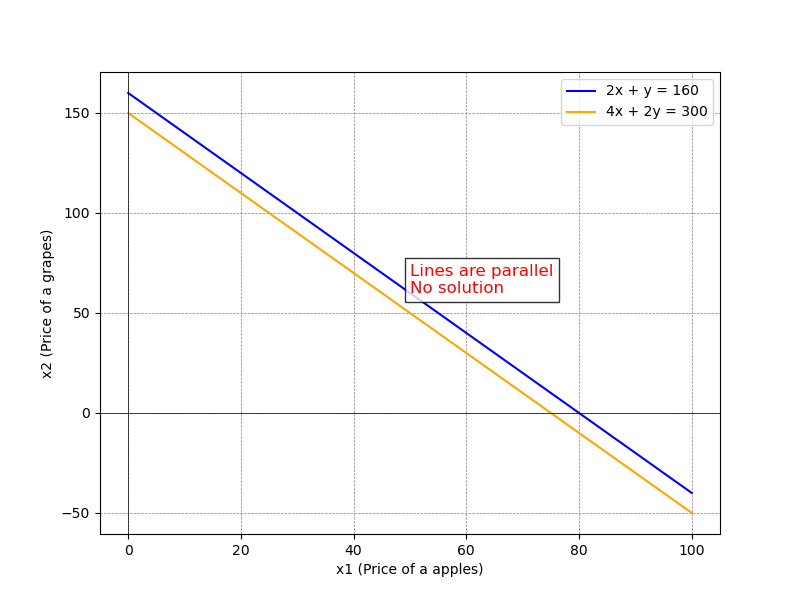
\includegraphics[width=\columnwidth]{figs/fig1.png}
		\caption{Solution of the system of linear equations}
		\label{stemplot}
	\end{figure}
	
\end{document}  
